
\documentclass[journal,10pt]{IEEEtran}
\usepackage{graphicx}
\usepackage{chngpage}
\usepackage{multirow}
\newcommand{\subparagraph}{}
% \usepackage [english]{babel}
% \usepackage [autostyle, english = american]{csquotes}
\usepackage{pgfplots}
\usepackage{pgfplotstable}
\usepackage{mathtools}
\usepackage{multicol}
\usepackage{titlesec}
\usepackage{gensymb}
\usepackage[justification=centering]{caption}
\usepackage{amsmath}
\usepackage{algorithm}
\usepackage[noend]{algpseudocode}
\usepackage{url}
\usepackage[final]{pdfpages}
%\usepackage{appendix}
\usepackage{float}
\usepackage{listings}
\usepackage{subfig}
 \usepackage[
    backend=biber,
    style=ieee,
  ]{biblatex}
\addbibresource{main.bib}
\usepackage[margin=0.75in]{geometry} % see geometry.pdf on how to lay out the page. There's lots.
\geometry{a4paper} % or letter or a5paper or ... etc
\setlength{\parskip}{0.5
em}



\definecolor{mygreen}{rgb}{0,0.6,0}
\definecolor{mygray}{rgb}{0.5,0.5,0.5}
\definecolor{mymauve}{rgb}{0.58,0,0.82}


\lstset{language=c,
breaklines=true,
commentstyle=\color{mygreen},
 keywordstyle=\color{blue},
 stringstyle=\color{mymauve},
 morecomment=[l]{//}}







% *** GRAPHICS RELATED PACKAGES ***
%
\ifCLASSINFOpdf
  % \usepackage[pdftex]{graphicx}
  % declare the path(s) where your graphic files are
  % \graphicspath{{../pdf/}{../jpeg/}}
  % and their extensions so you won't have to specify these with
  % every instance of \includegraphics
  % \DeclareGraphicsExtensions{.pdf,.jpeg,.png}
\else
  % or other class option (dvipsone, dvipdf, if not using dvips). graphicx
  % will default to the driver specified in the system graphics.cfg if no
  % driver is specified.
  % \usepackage[dvips]{graphicx}
  % declare the path(s) where your graphic files are
  % \graphicspath{{../eps/}}
  % and their extensions so you won't have to specify these with
  % every instance of \includegraphics
  % \DeclareGraphicsExtensions{.eps}
\fi
% graphicx was written by David Carlisle and Sebastian Rahtz. It is
% required if you want graphics, photos, etc. graphicx.sty is already
% installed on most LaTeX systems. The latest version and documentation
% can be obtained at: 
% http://www.ctan.org/tex-archive/macros/latex/required/graphics/
% Another good source of documentation is "Using Imported Graphics in
% LaTeX2e" by Keith Reckdahl which can be found at:
% http://www.ctan.org/tex-archive/info/epslatex/
%
% latex, and pdflatex in dvi mode, support graphics in encapsulated
% postscript (.eps) format. pdflatex in pdf mode supports graphics
% in .pdf, .jpeg, .png and .mps (metapost) formats. Users should ensure
% that all non-photo figures use a vector format (.eps, .pdf, .mps) and
% not a bitmapped formats (.jpeg, .png). IEEE frowns on bitmapped formats
% which can result in "jaggedy"/blurry rendering of lines and letters as
% well as large increases in file sizes.
%
% You can find documentation about the pdfTeX application at:
% http://www.tug.org/applications/pdftex





% *** MATH PACKAGES ***
%
%\usepackage[cmex10]{amsmath}
% A popular package from the American Mathematical Society that provides
% many useful and powerful commands for dealing with mathematics. If using
% it, be sure to load this package with the cmex10 option to ensure that
% only type 1 fonts will utilized at all point sizes. Without this option,
% it is possible that some math symbols, particularly those within
% footnotes, will be rendered in bitmap form which will result in a
% document that can not be IEEE Xplore compliant!
%
% Also, note that the amsmath package sets \interdisplaylinepenalty to 10000
% thus preventing page breaks from occurring within multiline equations. Use:
%\interdisplaylinepenalty=2500
% after loading amsmath to restore such page breaks as IEEEtran.cls normally
% does. amsmath.sty is already installed on most LaTeX systems. The latest
% version and documentation can be obtained at:
% http://www.ctan.org/tex-archive/macros/latex/required/amslatex/math/





% *** SPECIALIZED LIST PACKAGES ***
%
%\usepackage{algorithmic}
% algorithmic.sty was written by Peter Williams and Rogerio Brito.
% This package provides an algorithmic environment fo describing algorithms.
% You can use the algorithmic environment in-text or within a figure
% environment to provide for a floating algorithm. Do NOT use the algorithm
% floating environment provided by algorithm.sty (by the same authors) or
% algorithm2e.sty (by Christophe Fiorio) as IEEE does not use dedicated
% algorithm float types and packages that provide these will not provide
% correct IEEE style captions. The latest version and documentation of
% algorithmic.sty can be obtained at:
% http://www.ctan.org/tex-archive/macros/latex/contrib/algorithms/
% There is also a support site at:
% http://algorithms.berlios.de/index.html
% Also of interest may be the (relatively newer and more customizable)
% algorithmicx.sty package by Szasz Janos:
% http://www.ctan.org/tex-archive/macros/latex/contrib/algorithmicx/




% *** ALIGNMENT PACKAGES ***
%
%\usepackage{array}
% Frank Mittelbach's and David Carlisle's array.sty patches and improves
% the standard LaTeX2e array and tabular environments to provide better
% appearance and additional user controls. As the default LaTeX2e table
% generation code is lacking to the point of almost being broken with
% respect to the quality of the end results, all users are strongly
% advised to use an enhanced (at the very least that provided by array.sty)
% set of table tools. array.sty is already installed on most systems. The
% latest version and documentation can be obtained at:
% http://www.ctan.org/tex-archive/macros/latex/required/tools/


% IEEEtran contains the IEEEeqnarray family of commands that can be used to
% generate multiline equations as well as matrices, tables, etc., of high
% quality.




% *** SUBFIGURE PACKAGES ***
%\ifCLASSOPTIONcompsoc
%  \usepackage[caption=false,font=normalsize,labelfont=sf,textfont=sf]{subfig}
%\else
%  \usepackage[caption=false,font=footnotesize]{subfig}
%\fi
% subfig.sty, written by Steven Douglas Cochran, is the modeuion replacement
% for subfigure.sty, the latter of which is no longer maintained and is
% incompatible with some LaTeX packages including fixltx2e. However,
% subfig.sty requires and automatically loads Axel Sommerfeldt's caption.sty
% which will override IEEEtran.cls' handling of captions and this will result
% in non-IEEE style figure/table captions. To prevent this problem, be sure
% and invoke subfig.sty's "caption=false" package option (available since
% subfig.sty version 1.3, 2005/06/28) as this is will preserve IEEEtran.cls
% handling of captions.
% Note that the Computer Society format requires a larger sans serif font
% than the serif footnote size font used in traditional IEEE formatting
% and thus the need to invoke different subfig.sty package options depending
% on whether compsoc mode has been enabled.
%
% The latest version and documentation of subfig.sty can be obtained at:
% http://www.ctan.org/tex-archive/macros/latex/contrib/subfig/




% *** FLOAT PACKAGES ***
%
%\usepackage{fixltx2e}
% fixltx2e, the successor to the earlier fix2col.sty, was written by
% Frank Mittelbach and David Carlisle. This package corrects a few problems
% in the LaTeX2e kernel, the most notable of which is that in current
% LaTeX2e releases, the ordering of single and double column floats is not
% guaranteed to be preserved. Thus, an unpatched LaTeX2e can allow a
% single column figure to be placed prior to an earlier double column
% figure. The latest version and documentation can be found at:
% http://www.ctan.org/tex-archive/macros/latex/base/


%\usepackage{stfloats}
% stfloats.sty was written by Sigitas Tolusis. This package gives LaTeX2e
% the ability to do double column floats at the bottom of the page as well
% as the top. (e.g., "\begin{figure*}[!b]" is not normally possible in
% LaTeX2e). It also provides a command:
%\fnbelowfloat
% to enable the placement of footnotes below bottom floats (the standard
% LaTeX2e kernel puts them above bottom floats). This is an invasive package
% which rewrites many portions of the LaTeX2e float routines. It may not work
% with other packages that modify the LaTeX2e float routines. The latest
% version and documentation can be obtained at:
% http://www.ctan.org/tex-archive/macros/latex/contrib/sttools/
% Do not use the stfloats baselinefloat ability as IEEE does not allow
% \baselineskip to stretch. Authors submitting work to the IEEE should note
% that IEEE rarely uses double column equations and that authors should try
% to avoid such use. Do not be tempted to use the cuted.sty or midfloat.sty
% packages (also by Sigitas Tolusis) as IEEE does not format its papers in
% such ways.
% Do not attempt to use stfloats with fixltx2e as they are incompatible.
% Instead, use Morten Hogholm'a dblfloatfix which combines the features
% of both fixltx2e and stfloats:
%
% \usepackage{dblfloatfix}
% The latest version can be found at:
% http://www.ctan.org/tex-archive/macros/latex/contrib/dblfloatfix/




%\ifCLASSOPTIONcaptionsoff
%  \usepackage[nomarkers]{endfloat}
% \let\MYoriglatexcaption\caption
% \renewcommand{\caption}[2][\relax]{\MYoriglatexcaption[#2]{#2}}
%\fi
% endfloat.sty was written by James Darrell McCauley, Jeff Goldberg and 
% Axel Sommerfeldt. This package may be useful when used in conjunction with 
% IEEEtran.cls'  captionsoff option. Some IEEE journals/societies require that
% submissions have lists of figures/tables at the end of the paper and that
% figures/tables without any captions are placed on a page by themselves at
% the end of the document. If needed, the draftcls IEEEtran class option or
% \CLASSINPUTbaselinestretch interface can be used to increase the line
% spacing as well. Be sure and use the nomarkers option of endfloat to
% prevent endfloat from "marking" where the figures would have been placed
% in the text. The two hack lines of code above are a slight modification of
% that suggested by in the endfloat docs (section 8.4.1) to ensure that
% the full captions always appear in the list of figures/tables - even if
% the user used the short optional argument of \caption[]{}.
% IEEE papers do not typically make use of \caption[]'s optional argument,
% so this should not be an issue. A similar trick can be used to disable
% captions of packages such as subfig.sty that lack options to turn off
% the subcaptions:
% For subfig.sty:
% \let\MYorigsubfloat\subfloat
% \renewcommand{\subfloat}[2][\relax]{\MYorigsubfloat[]{#2}}
% However, the above trick will not work if both optional arguments of
% the \subfloat command are used. Furthermore, there needs to be a
% description of each subfigure *somewhere* and endfloat does not add
% subfigure captions to its list of figures. Thus, the best approach is to
% avoid the use of subfigure captions (many IEEE journals avoid them anyway)
% and instead reference/explain all the subfigures within the main caption.
% The latest version of endfloat.sty and its documentation can obtained at:
% http://www.ctan.org/tex-archive/macros/latex/contrib/endfloat/
%
% The IEEEtran \ifCLASSOPTIONcaptionsoff conditional can also be used
% later in the document, say, to conditionally put the References on a 
% page by themselves.




% *** PDF, URL AND HYPERLINK PACKAGES ***
%
%\usepackage{url}
% url.sty was written by Donald Arseneau. It provides better support for
% handling and breaking URLs. url.sty is already installed on most LaTeX
% systems. The latest version and documentation can be obtained at:
% http://www.ctan.org/tex-archive/macros/latex/contrib/url/
% Basically, \url{my_url_here}.




% *** Do not adjust lengths that control margins, column widths, etc. ***
% *** Do not use packages that alter fonts (such as pslatex).         ***
% There should be no need to do such things with IEEEtran.cls V1.6 and later.
% (Unless specifically asked to do so by the journal or conference you plan
% to submit to, of course. )


% correct bad hyphenation here
\hyphenation{op-tical net-works semi-conduc-tor}

\graphicspath{{imgs/}{}}
\begin{document}
%
% paper title
% Titles are generally capitalized except for words such as a, an, and, as,
% at, but, by, for, in, nor, of, on, or, the, to and up, which are usually
% not capitalized unless they are the first or last word of the title.
% Linebreaks \\ can be used within to get better formatting as desired.
% Do not put math or special symbols in the title.
\title{ELEN 4020 Lab 2: OpenMP and Pthreads}
%
%
% author names and IEEE memberships
% note positions of commas and nonbreaking spaces ( ~ ) LaTeX will not break
% a structure at a ~ so this keeps an author's name from being broken across
% two lines.
% use \thanks{} to gain access to the first footnote area
% a separate \thanks must be used for each paragraph as LaTeX2e's \thanks
% was not built to handle multiple paragraphs
%
%\onecolumn
\author{Junaid Dawood (1094837), Xongile Nghatsane (1110680), Marissa van Wyngaardt (719804)}% <-this % stops a space



\maketitle

% As a general rule, do not put math, special symbols or citations
% in the abstract or keywords.

\begin{abstract}
This report discusses the parallelisation of matrix transposition algorithms in C, using OpenMP and Pthreads. The implemented algorithms include a naive element-wise swapping approach, a diagonal based row-column swap approach, and a block based approach. From a comparative analysis of the \textit{runtimes} of the implemented algorithms, it was found that the Pthreads implementation of the block based algorithm yielded the best performance once the sizes of input matrices are sufficiently large. This is thought to be due to the even work-sharing implemented for this approach, that was not achieved elsewhere. Additional throttling has been identified in the implementations and has been linked to false sharing and cache misses.
\end{abstract}

\IEEEpeerreviewmaketitle

\section{Introduction}

This document discusses the implementation of three matrix transposition algorithms in C. Initially, these are implemented serially; they are subsequently parallelised through the use of OpenMP and Pthreads \cite{omp,pthreads}. This report also discusses tradeoffs with respect to parallelisation, in terms of computation times. In particular, the point at which the communication overhead of parallelisation is outweighed by the performance gain of said parallelisation is a key concern of this lab exercise.

%consider revising

\section {Structs and Helper Functions}

This lab exercise involved the reuse of a rank 2 tensor struct created for the first lab exercise. This struct is used to store matrices, and metadata i.e. the dimensions of the matrix. Additional helper functions for the initialisation of the contents of the tensor, and the freeing of memory dynamically allocated for their content are implemented.

Additionally, other structs are required for achieving parallelisation using Pthreads; in order to work-share between threads. That is, these structs contain additional data which indicates to the transposition algorithm the \textit{segment} of the matrix which is to be parallelised by a certain thread.





\section{Transposition Algorithms}

This section describes the three matrix transposition algorithms implemented, which were ultimately parallelised. The algorithms implemented consist of a naive approach, a diagonal row-per-column transposition, and a block based transposition with intra-block transposition and inter-block position swapping. All of the algorithms are constrained to $O(1)$ space complexity.

It is important to note that the naive approach and the diagonal approach are very similar, and in the case of a serial implementation, are identical. Hence, differences in implementation only manifest in the way in which they are parallelised. The pseudocode for all the algorithms, including parallelisations, can be found at the end of this document.

\subsection{Naive Approach}
The naive approach involves iterating through every cell above the main diagonal. The contents of the cells are then swapped with the corresponding cells in the lower half of the matrix as shown in the diagram below.

When parallelised, there would ideally be a thread allocated to each pair of elements to be swapped; in order for the implementation to remain within the philosophy of the naive approach.

\begin{figure}[H]
    \centering
    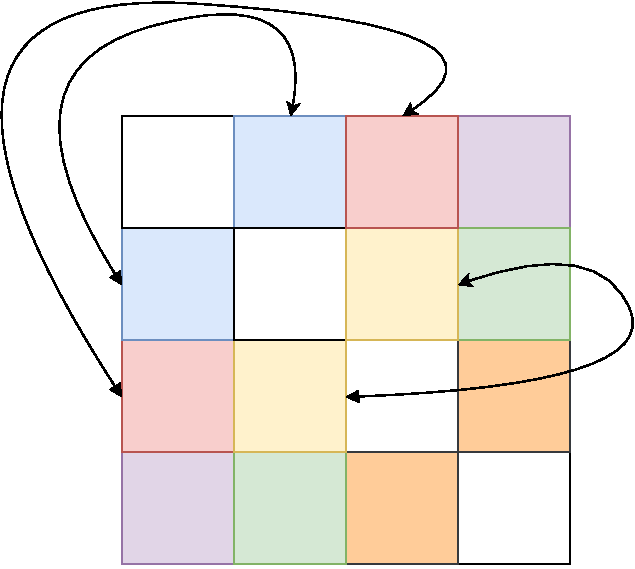
\includegraphics[width=0.35\textwidth]{naive.pdf}
    \caption{Naive matrix transposition algorithm.}
    \label{fig:my_label}
\end{figure}

\subsection{Diagonal Approach}
The diagonal approach is similar to the naive approach as mentioned above. The difference lies in the manner of the iteration and thus the order of the swapping. That is, in the diagonal approach it is the diagonal which is iterated along: with a partial transposition occurring at each element on the diagonal. Each element on the diagonal naturally exists as the intersection between a column and a row: the swapping of said row and column is what constitutes the partial transposition, as shown below.

\begin{figure}[H]
    \centering
    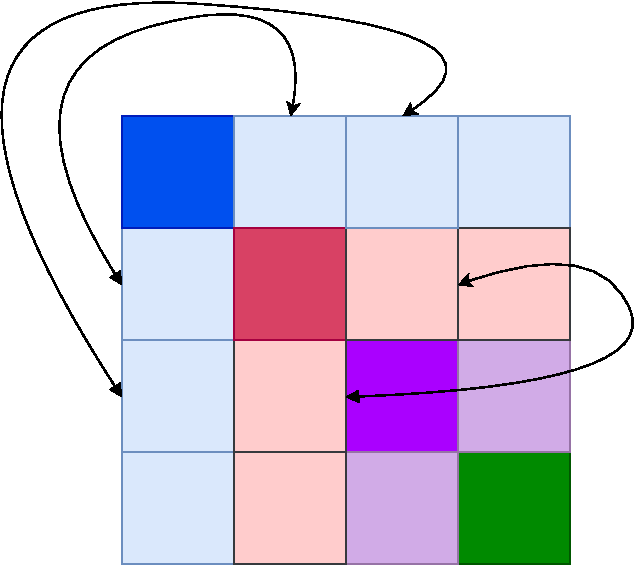
\includegraphics[width=0.35\textwidth]{diag.pdf}
    \caption{Diagonal matrix transposition algorithm.}
    \label{fig:my_label}
\end{figure}


\clearpage
That said, within a serial implementation the distinction of iterating along each cell compared to each cell on the diagonal is lost; thus it becomes equivalent to the naive approach. In a parallel approach, the swapping of rows with columns would be handled by a single thread per diagonal; such that this method becomes distinct from the naive approach.

\subsection{Block Approach}
In this approach, the matrix to be transposed is decomposed into 2x2 sub-matrices (blocks). These blocks are individually transposed and then they are swapped with the corresponding blocks below or above the main diagonal. The blocks on the main diagonal are simply transposed, and do not go through any swapping process. Naturally, the use of 2x2 blocks is a limiting factor in that it can only partition matrices of even dimensions.



This can be seen in the diagram shown below: note the individual internal transpositions of the 2x2 blocks, and the subsequent swapping with like-coloured blocks. The 2x2 blocks which exist along the diagonal of the matrix naturally only require the internal transposition step and not the swapping step. 

\begin{figure}[H]
    \centering
    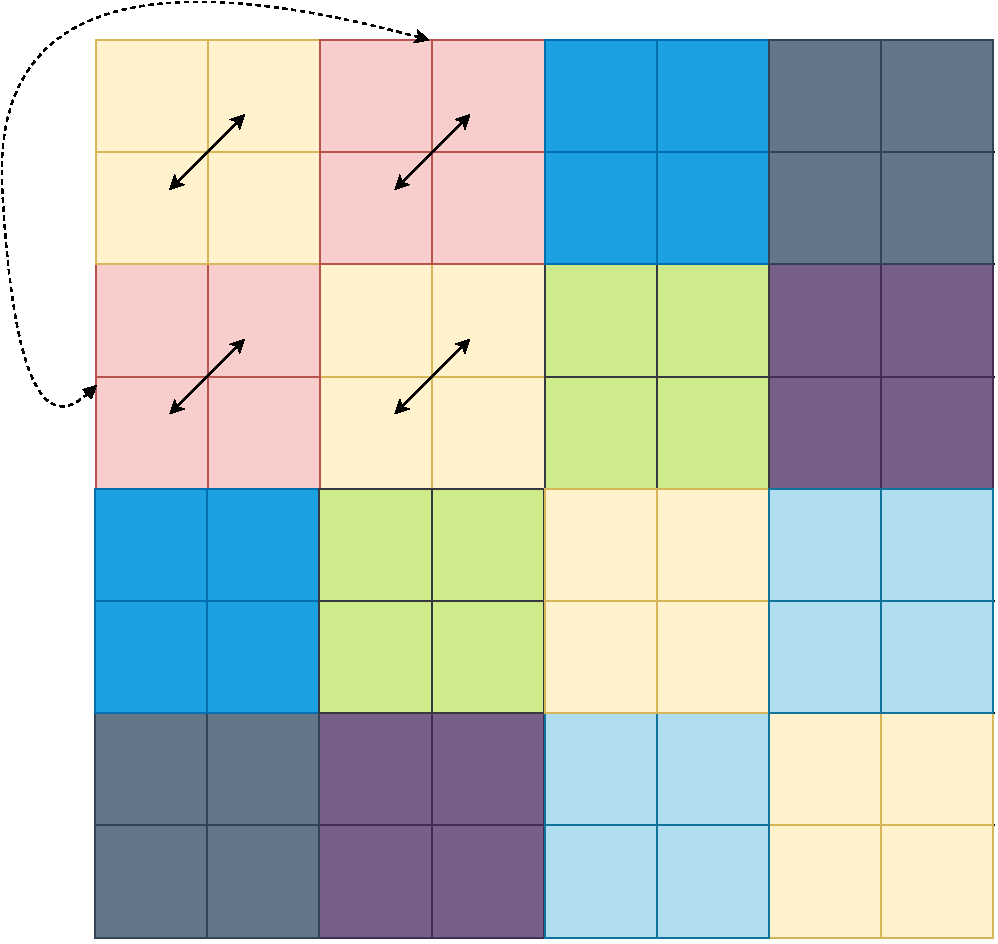
\includegraphics[width=0.35\textwidth]{block.pdf}
    \caption{Block-based matrix transposition algorithm.}
    \label{fig:my_label}
\end{figure}

A simple parallelisation of this approach would be to allocate a thread to each block pair being processed. Thus, this thread would transpose the individual blocks, as well as perform the swap of the two blocks.


\section{OpenMP Parallelisation}

This section discusses the parallelisation of the aforementioned serial transposition algorithms using OpenMP. This is done entirely through the use of compiler directives, specifically those used for the parallelisation of for loops.


\subsection{Naive Approach}
The parallelisation of the naive approach is achieved through essentially assigning a thread to each cell-swap operation that is required for the transposition. This is achieved by parallelising the outer \textit{for} loop such that each thread is assigned a near equal number of cell swaps. There are $\frac{N(N+1)}{2}$ swap operations in total, shared across $M$ threads i.e. $\frac{N(N+1)}{2M}$ swaps per thread ideally.

Parallelising the outer loop, instead of the inner loop, allows for a far smaller number of fork-join operations to be used in the program's execution. Parallelising the inner loop would require fork-join operations on a per row basis, resulting in far more overhead than the chosen method. Similarly, the use of nested parallelism makes for a less efficient solution; this is a much more time consuming way in which to implement work sharing as there is an overhead incurred for each swap operation \cite{Chapter356:online}. %Because of these consequences, 

\subsection{Diagonal Approach}
The parallelisation of the diagonal approach corresponds to the assignment of a thread to each diagonal element of the matrix; such that a thread is tasked with all of the row-column swaps corresponding to the diagonal element it is assigned to. This is done simply by using OpenMP to parallelise the outer \textit{for} loop of the serial implementation.

Unlike the naive approach, a thread is not assigned a \textit{chunk} of elements to swap, instead a single thread is responsible for all of the associated swaps of its row(s) and column(s). In addition, whilst it can be said that the number of swaps per thread is constant in the naive case, this is not true of the diagonal implementation, That is, threads allocated elements further along the diagonal will inherently have to do fewer swaps than those allocated elements earlier in the diagonal.

\subsection{Block Approach}

The parallelisation of the block approach using OpenMP would ideally involve assigning threads to an even number of block-transposition and block-swap operations. However, this is not easily achieved using OpenMP; for similar reasons to the diagonal approach.


That is, OpenMP is used to parallelise the outer \textit{for} loop of the serial implementation. In this way, each thread is given an equal number of blocks to transpose and swap. In total, given the use of 2x2 blocks, the total number of blocks is given by $noBlocks=\frac{L(L+1)}{2}$, where $L=\frac{N}{2}$ for a $N\times N$ matrix.



\section{Pthreads Parallelisation}
The parallelisation of the serial implementations of matrix transposition using Pthreads is more involved than when using OpenMP. That is, the explicit manual definition of the work-sharing is required when using Pthreads, which is not the case when using OpenMP.

Generally, this involves manually splitting work into \textit{chunks}, and assigning said chunks to individual threads. This is generally done by defining the scope of a thread's work, placing the scope defining variables into a \textit{struct} along with a reference to the original matrix. This \textit{struct} is then passed to the relevant transposition method upon invocation.% It follows that the parallelisation of the naive approach

\subsection{Diagonal Approach}

As per the above discussion, parallelisation of the diagonal transposition approach involves defining the manner in which work is shared amongst threads. This is achieved by assigning each thread a number of diagonal elements, based on the size of the matrix and the number of threads, such that each thread is allocated the same number of diagonal elements.



Thus, each thread is assigned a start and end row in the matrix, as per the snippet below. Each thread handles each diagonal element it is responsible for; performing the row-column swaps for each diagonal.

\begin{lstlisting}
typedef struct forDiagonal
{
    rank2Tensor* srcMat;
	int start;
	int end;
} forDiag;
\end{lstlisting}


This does not achieve equal work-sharing due to different diagonal elements implying a different number of swap operations, as is the case with the OpenMP parallelisation.


\subsection{Block Approach}
The parallelisation of the block transposition using Pthreads is more complex than the parallelisation of the diagonal method. That said, the basic premise remains the same: each thread is assigned a certain number of blocks which it is responsible for; performing the necessary intra-block transpositions and subsequent block swaps. The listing below shows the \textit{struct} passed on a per-thread basis, to the block transposition function.


\begin{lstlisting}
typedef struct forBlock
{
	rank2Tensor* srcMat;
	int startBlock;
	int noBlocks;

} forBlock;
\end{lstlisting}

The nature of the block implementation requires a coordinate mapping system which relates the rows and columns of the original matrix to a number of sequenced blocks. This is done within the called function, once per thread, and as such, this conversion overhead is not thought to be significant.

%\onecolumn
\section{Results and Discussion}

Tests were conducted on a per algorithm basis, for each parallelisation method used. In addition, the serial implementations of the algorithms were also tested, for comparison. Testing consisted of supplying matrices of increasing size to the algorithms, measuring the time taken for the algorithms to complete the transpositions.

Timing was done using OpenMP's \textit{get wtime} function; being used before and after calls to the algorithms in order to obtain their completion times. This was used in all implementations i.e. serial, parallel (Pthreads), and parallel (OpenMP), in order to ensure a fair timekeeping process across all tests.

The test machine that the code was run on had the following specifications:

\begin{itemize}
    \item CPU: Intel i5 8350u (4C 8T) 3.6~GHz turbo frequency (256~kB L1, 1~MB L2, 6~MB L3) \cite{8350u}.
    \item RAM: 16 GB \@ 2400~MHz
\end{itemize}


The tables and graphs shown in this section are automatically generated in \LaTeX from the output CSV files from running the respective implementations. This is to ensure that data is not compared across multiple test runs.


\begin{table}[h]
\begin{adjustwidth}{-0cm}{}
\centering
\caption{Results for Serial Implementation (Times in seconds)}
\pgfplotstabletypeset[
      multicolumn names, % allows to have multicolumn names
      col sep=comma, % the seperator in our .csv file
      display columns/0/.style={
		column name=$Matrix Size$, % name of first column
		column type={S},string type},  % use siunitx for formatting
      display columns/1/.style={
		column name=$Naive Approach$,
		column type={S},string type},
		display columns/2/.style={
		column name=$Diagonal Approach$,
		column type={S},string type},
		display columns/3/.style={
		column name=$Block Approach$,
		column type={S},string type}
    ]{serial.csv} % filename/path to file
    \end{adjustwidth}

\end{table}




\begin{table}[h]
\begin{adjustwidth}{-0cm}{}
\centering
\caption{Results for OMP Parallelisation (Times in seconds)}

\pgfplotstabletypeset[
      multicolumn names, % allows to have multicolumn names
      col sep=comma, % the seperator in our .csv file
      display columns/0/.style={
		column name=$Matrix Size$, % name of first column
		column type={S},string type},  % use siunitx for formatting
      display columns/1/.style={
		column name=$Naive Approach$,
		column type={S},string type},
		display columns/2/.style={
		column name=$Diagonal Approach$,
		column type={S},string type},
		display columns/3/.style={
		column name=$Block Approach$,
		column type={S},string type}
    ]{omp.csv} % filename/path to file
    
    
\end{adjustwidth}    
\end{table}





\begin{table}[h]
\centering
\caption{Results for Pthreads Parallelisation (Times in seconds)}
\pgfplotstabletypeset[
      multicolumn names, % allows to have multicolumn names
      col sep=comma, % the seperator in our .csv file
      display columns/0/.style={
		column name=$Matrix Size$, % name of first column
		column type={S},string type},  % use siunitx for formatting
		display columns/1/.style={
		column name=$Diagonal Approach$,
		column type={S},string type},
		display columns/2/.style={
		column name=$Block Approach$,
		column type={S},string type}
    ]{pthreads.csv} % filename/path to file
\end{table} 



%data is saved in matsize,naive,diag,block
%except for pthreads, which does not have naive
\begin{figure}[H]
  \begin{center}
    \begin{tikzpicture}
      \begin{axis}[
          width= 0.8\linewidth,
          xlabel= Matrix size $N_0$, % Set the labels
          ylabel= Time (s),
          legend style={draw=none},
          legend pos=north west,
          xmin=0,
          ymin=0
        ]
        \addplot table [ x index= {0},y index={1}, col sep=comma,mark=none] {serial.csv};
        \addplot table [ x index= {0},y index={1}, col sep=comma,mark=none] {omp.csv};
        \legend{Serial,OpenMP}
      \end{axis}
    \end{tikzpicture}
    \caption{Comparison of Naive Implementations of matrix transpositions.}
  \end{center}
\end{figure}


\begin{figure}[H]
  \begin{center}
    \begin{tikzpicture}
      \begin{axis}[
          width= 0.8\linewidth,
          xlabel= Matrix size $N_0$, % Set the labels
          ylabel= Time (s),
          legend style={draw=none},
          legend pos=north west,
          xmin=0,
          ymin=0
        ]
        \addplot table [ x index= {0},y index={2}, col sep=comma,mark=none] {serial.csv};
        \addplot table [ x index= {0},y index={2}, col sep=comma,mark=none] {omp.csv};
        \addplot table [ x index= {0},y index={1}, col sep=comma,mark=none] {pthreads.csv};
        
        \legend{Serial,OpenMP,Pthread}
      \end{axis}
    \end{tikzpicture}
    \caption{Comparison of Diagonal Implementations of matrix transpositions.}
  \end{center}
\end{figure}


\begin{figure}[H]
  \begin{center}
    \begin{tikzpicture}
      \begin{axis}[
          width= 0.8\linewidth,
          xmin=0,
          xlabel= Matrix size $N_0$, % Set the labels
          ylabel= Time (s),
          legend style={draw=none},
          legend pos=north west,
            xmin=0,
          ymin=0
        ]
        \addplot table [ x index= {0},y index={3}, col sep=comma,mark=none] {serial.csv};
        \addplot table [ x index= {0},y index={3}, col sep=comma,mark=none] {omp.csv};
        \addplot table [ x index= {0},y index={2}, col sep=comma,mark=none] {pthreads.csv};
        
        \legend{Serial,OpenMP,Pthread}
      \end{axis}
    \end{tikzpicture}
    \caption{Comparison of Block Implementations of matrix transpositions.}
  \end{center}
\end{figure}

%\twocolumn

\subsection{Discussion}

From the results, it is clear that the overhead involved in forking and joining of threads causes the performance of serial and parallel approaches to be similar for small matrices. As far as comparisons between parallel implementations, it is clear that the block approach begins to perform better than the diagonal approach beyond a threshold. This is thought to be due to the more efficient work-sharing implied by the block approach. 

In addition, there is an apparent divergence between the performance of the block implementations between the OpenMP and Pthreads implementations. This is thought to be due to the fact that the manual nature of the Pthreads implementation allowed for even work-sharing, whereas the OpenMP approach did not. This is discussed further below.


There are various issues present within the current (parallel) implementations that manifest in the trends present in the results. The first obvious fault is the lack of (near) even work-sharing between threads in some implementations; specifically, block and diagonal (OpenMP) and diagonal (Pthreads). As a result, the threads which are allocated more of the work would ultimately take the longest to complete their work. This time would naturally be longer than the time taken if work-sharing were implemented evenly.


Another issue present within the current implementations is false sharing \cite{false}. This refers to scenarios which involve threads which access independent variables which share the same cache line. When one thread writes over their independent variable, it is required that the other thread invalidates its copy of the cache line, having to copy the new (altered) cache line in order to continue. This is especially problematic if each thread is making several alterations to the cache line. In addition, as the number of threads increases, it naturally follows that this cache invalidation could become a more common occurrence. 

The current implementations offer no mechanisms with which to prevent this. Given that this exercise is mainly concerned with matrices, it follows that false sharing is a common occurrence if not accounted for. That said, these algorithms achieve $O(1)$ space complexity, as per the current implementation; achieving this whilst avoiding false sharing would be a difficult exercise.

Lastly, caching and more specifically cache misses are an important factor to consider when discussing matrix transposition implementations \cite{cmiss}. This is to the extent that there have been studies into cache efficient matrix transposition implementations \cite{c1,c2}. A cache miss refers to a thread failing to find some variable within the lowest cache level, causing the thread to have to fetch the data from a higher cache level, eventually reaching main memory if the data is not found at any cache level. Generally speaking, the inter-level latencies increase whilst travelling up the hierarchy e.g. from L1 to L2 cache the latency is minimal compared to the L3 cache to main memory latency. %Cache efficient design requires significant forethought and 


%%uneven work sharing
%false sharing, cache misses etc.
%\newpage

\section{Conclusion}
Three implementations of matrix transposition algorithms have been presented. This has been done with specific reference to the parallelisation of these methods, implemented in C. In doing so, the use of OpenMP and Pthreads as tools for achieving the parallelisation of the algorithms has also been presented, alongside a performance comparison of the two on a per algorithm basis. It has been shown that a naive method has a clear advantage within a naive implementation. However, when parallelised, the block approach quickly begins to outperform both the naive and diagonal approaches, as the size of the input matrices increases.

%\renewcommand*{\bibfont}{\small}
\clearpage
\onecolumn
\printbibliography

\clearpage

\onecolumn
\section*{Pseudocode}
\subsection*{Serial}
\pagenumbering{gobble}

\begin{algorithm}
\caption{Naive Approach (Serial)}\label{euclid}
\begin{algorithmic}[1]
\Procedure{naiveTransposition}{rank2Tensor t1}
\State $\textit{t1} \gets \textit{first rank 2 tensor}$


\For{i=0..t1.rows}
\For{j=0..(i-1)}
\State swap(t1[i][[j],t2[j][i])
\EndFor
\EndFor



\EndProcedure
\end{algorithmic}
\end{algorithm}


\begin{algorithm}
\caption{Diagonal Approach (Serial)}\label{euclid}
\begin{algorithmic}[1]
\Procedure{diagonalTransposition}{rank2Tensor t1}
\State $\textit{t1} \gets \textit{first rank 2 tensor}$


\For{i=0..t1.rows}
\For{j=i..t1.cols}
\State swap(t1[i][[j],t2[j][i])
\EndFor
\EndFor



\EndProcedure
\end{algorithmic}
\end{algorithm}


\begin{algorithm}
\caption{Block Approach (Serial)}\label{euclid}
\begin{algorithmic}[1]
\Procedure{blockTransposition}{rank2Tensor t1}
\State $\textit{t1} \gets \textit{first rank 2 tensor}$


\For{i=0..blockCount}
\State Transpose block i
\State Transpose opposite block
\State Swap block i and opposite block
\EndFor



\EndProcedure
\end{algorithmic}
\end{algorithm}


\clearpage

\subsection*{OpenMP}
\begin{algorithm}
\caption{Diagonal Approach (OpenMP)}\label{euclid}
\begin{algorithmic}[1]
\Procedure{diagonalTransposition}{rank2Tensor t1}
\State $\textit{t1} \gets \textit{first rank 2 tensor}$

\State 	\#pragma omp parallel for
\For{i=0..t1.rows}
\For{j=i..t1.cols}
\State swap(t1[i][[j],t2[j][i])
\EndFor
\EndFor



\EndProcedure
\end{algorithmic}
\end{algorithm}



\begin{algorithm}
\caption{Block Approach (OpenMP)}\label{euclid}
\begin{algorithmic}[1]
\Procedure{diagonalTransposition}{rank2Tensor t1}
\State $\textit{t1} \gets \textit{first rank 2 tensor}$

\State \#pragma omp parallel for
\For{i=0..t1.rows}
\For{j=i..t1.cols}
\State swap(t1[i][[j],t2[j][i])
\EndFor
\EndFor



\EndProcedure
\end{algorithmic}
\end{algorithm}



\begin{algorithm}
\caption{Block Approach (OpenMP)}\label{euclid}
\begin{algorithmic}[1]
\Procedure{blockTransposition}{rank2Tensor t1}
\State $\textit{t1} \gets \textit{first rank 2 tensor}$

\#pragma omp parallel for
\For{i=0..blockCount}
\State Transpose block i
\State Transpose opposite block
\State Swap block i and opposite block
\EndFor



\EndProcedure
\end{algorithmic}
\end{algorithm}
\clearpage
\subsection*{PThreads}


\begin{algorithm}
\caption{Diagonal Approach (Pthreads)}\label{euclid}
\begin{algorithmic}[1]

\Procedure{WorkAssignment}{}

\State $\textit{threads} \gets \textit{list of threads}$
\State ${N_0} \gets \textit{matrix row count}$

\State $\textit{threadCount} \gets \textit{number of available threads}$


perThread=$N_0$/threadcount
\For{i=0..threadCount-1}
 \State   threads[i].startRow=i*perThread
  \State  threads[i].startRow=(i+1)*perThread
\EndFor

threads[threadCount-1].endRow=$N_0$

\EndProcedure



\Procedure{diagonalTransposition}{rank2Tensor t1,startRow,endRow}
\State $\textit{t1} \gets \textit{first rank 2 tensor}$
\State $\textit{startRow} \gets \textit{start of thread's diagonals}$
\State $\textit{endRow} \gets \textit{end of thread's diagonals}$

\For{i=startRow..endRow}
\For{j=i..t1.cols}
\State swap(t1[i][[j],t2[j][i])
\EndFor
\EndFor



\EndProcedure
\end{algorithmic}
\end{algorithm}



\begin{algorithm}
\caption{Block Approach (Pthreads)}\label{euclid}
\begin{algorithmic}[1]

\Procedure{WorkAssignment}{}

\State $\textit{threads} \gets \textit{list of threads}$
\State ${N_0} \gets \textit{matrix row count}$

\State $\textit{threadCount} \gets \textit{number of available threads}$

blockCount=($N_0$/2)($N_0$/2 +1)/2

perThread=blockCount/threadcount
\For{i=0..threadCount-1}
 \State   threads[i].startBlock=i*perThread
  \State  threads[i].endBlock=(i+1)*perThread
\EndFor

threads[threadCount-1].endBlock=blockCount

\EndProcedure



\Procedure{blockTransposition}{rank2Tensor t1,startBlock,endBlock}
\State $\textit{t1} \gets \textit{first rank 2 tensor}$
\State $\textit{startRow} \gets \textit{start of thread's diagonals}$
\State $\textit{endRow} \gets \textit{end of thread's diagonals}$

\For{blockNo = startBlock..endBlock}
\State transpose(blockNo)
\State transpose(alternateBlock)
\State swap blockNo and alternateBlock
\EndFor




\EndProcedure
\end{algorithmic}
\end{algorithm}



\clearpage

\newrefsection
\pagenumbering{arabic}
\onecolumn 
%\setlength{\parskip}{0.6em}




\ifCLASSOPTIONcaptionsoff
  \newpage
\fi



% trigger a \newpage just before the given reference
% number - used to balance the columns on the last page
% adjust value as needed - may need to be readjusted if
% the document is modified later
%\IEEEtriggeratref{8}
% The "triggered" command can be changed if desired:
%\IEEEtriggercmd{\enlargethispage{-5in}}

% references section

% can use a bibliography generated by BibTeX as a .bbl file
% BibTeX documentation can be easily obtained at:
% http://www.ctan.org/tex-archive/biblio/bibtex/contrib/doc/
% The IEEEtran BibTeX style support page is at:
% http://www.michaelshell.org/tex/ieeetran/bibtex/
%\bibliographystyle{IEEEtran}
% argument is your BibTeX string definitions and bibliography database(s)
%\bibliography{IEEEabrv,../bib/paper}
%
% <OR> manually copy in the resultant .bbl file
% set second argument of \begin to the number of references
% (used to reserve space for the reference number labels box)
%\begin{thebibliography}{1}

%\bibitem{IEEEhowto:kopka}

% H.~Kopka and P.~W. Daly, \emph{A Guide to \LaTeX}, 3rd~ed.\hskip 1em plus
%   0.5em minus 0.4em\relax Harlow, England: Addison-Wesley, 1999.

%\end{thebibliography}

% biography section
% 
% If you have an EPS/PDF photo (graphicx package needed) extra braces are
% needed around the contents of the optional argument to biography to prevent
% the LaTeX parser from getting confused when it sees the complicated
% \includegraphics command within an optional argument. (You could create
% your own custom macro containing the \includegraphics command to make things
% simpler here.)
%\begin{IEEEbiography}[{\includegraphics[width=1in,height=1.25in,clip,keepaspectratio]{mshell}}]{Michael Shell}
% or if you just want to reserve a space for a photo:

% \begin{IEEEbiography}
% Biography text here.
% \end{IEEEbiography}

% if you will not have a photo at all:
% \begin{IEEEbiographynophoto}{John Doe}
% Biography text here.
% \end{IEEEbiographynophoto}

% insert where needed to balance the two columns on the last page with
% biographies
%\newpage

% \begin{IEEEbiographynophoto}{Jane Doe}
% Biography text here.
% \end{IEEEbiographynophoto}

% You can push biographies down or up by placing
% a \vfill before or after them. The appropriate
% use of \vfill depends on what kind of text is
% on the last page and whether or not the columns
% are being equalized.

%\vfill

% Can be used to pull up biographies so that the bottom of the last one
% is flush with the other column.
%\enlargethispage{-5in}



% that's all folks
\end{document}